\documentclass[preview]{standalone}
\usepackage{tikz}
\usetikzlibrary{arrows}

\begin{document}
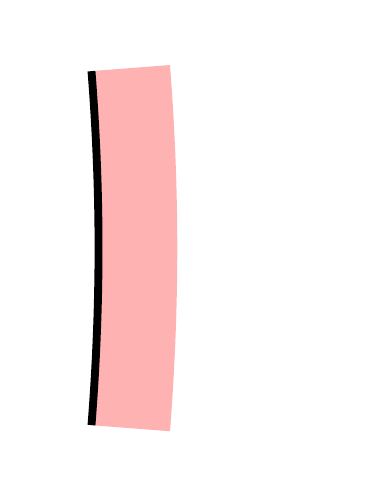
\begin{tikzpicture}[scale=1,
rotate = 180,
stretch/.style={color=red!30, line width=1cm},
solid/.style={line width=1mm}]

\def\pressure{10}
\def\hx{5}	
\def\hy{1}  % change only with line width of stretch
\def\yshift{1.5}	% Shift zwischenden principles
\pgfmathsetmacro{\hyh}{.5*\hy}
\pgfmathsetmacro{\hxh}{\hx/2}



\path[clip] (-2.7,\hxh+.3)rectangle++(4.1,-\hx-.6);


\pgfmathsetmacro{\alp}{90*\pressure/200}
\pgfmathsetmacro{\alph}{\alp*.5}

\def\pi{3.1416}
\pgfmathsetmacro{\r}{\hx/\alp*180/\pi*.9}
\pgfmathsetmacro{\rh}{\r*.5}
%\pgfmathsetmacro{\hyhh}{\hyh*.5}


% Bended
\draw[stretch] (0,0)arc(180:180-\alp:\rh+\hyh);
\draw[stretch] (0,0)arc(180:180+\alp:\rh+\hyh);

\draw[solid] (+\hyh,0)arc(180:180-\alp:\rh);
\draw[solid] (+\hyh,0)arc(180:180+\alp:\rh);




\end{tikzpicture}
\end{document}